%*******************************************************************************
%****************************** Fifth Chapter *********************************
%*******************************************************************************

\chapter{Cosmic $\mu$ Telescopes}\label{chp:cosmicMuTelescopes}

\ifpdf
    \graphicspath{{Chapter5/Figs/Raster/}{Chapter5/Figs/PDF/}{Chapter5/Figs/}}
\else
    \graphicspath{{Chapter5/Figs/Vector/}{Chapter5/Figs/}}
\fi

\section{Overview Of Cosmic $\mu$ Tomography}\label{sec:cosMuOverview}
Cosmic $\mu$ tomography can be split into two distinct types. Two-sided cosmic $\mu$ tomography measures the incoming $\mu$ angles and outgoing $\mu$ angles over a given area with an object of interest to be imaged as shown by figure \ref{fig:twoSidedCosmicMuonTomographySchults}. This approach allows for vertex reconstruction and measures cosmic $\mu$ scattering thus giving a detailed interior image of the object being imaged \cite{schultz_2007}. This approach has been used to analyse nuclear waste \cite{jonkmans2013nuclear} and even imaging the Fukushima Daiichi reactors \cite{miyadera2013imaging}. However, as figure \ref{fig:twoSidedCosmicMuonTomographySchults} shows the  detectors are typically much larger or of similar size to the object that they are attempting to image. So whilst this technique would yield a very accurate breakdown of the internal structure of any given object it would not be suitable in all cases. For example, if the object of interest were significantly larger than the detectors then only a small portion of it could be analysed. Further, this technique doesn't work if there's only one detector array. For the VIDARR prototype deployed at Wylfa, it was both significantly smaller than the reactor buildings and only one detector was deployed. As a result, one-sided cosmic $\mu$ tomography will be used from this point onward. 

\begin{figure}[!h]
 \centering
 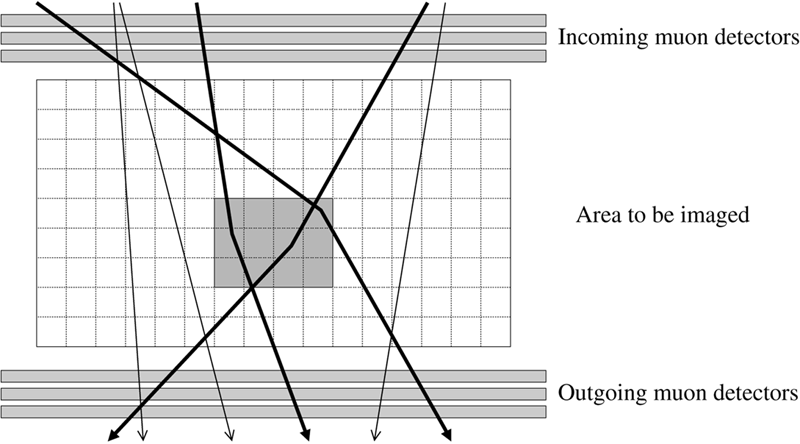
\includegraphics[width=0.7\linewidth]{Chapter5/Figs/Raster/twoSidedCosmicMuon_schults2007.png}
 \captionof{figure}{A side-on view of two-sided cosmic $\mu$ tomography the detectors are of similar size or larger than the object that is being measured in order to make coincided measurements using cosmic $\mu$ seen in the scattered (black) cosmic $\mu$. From \cite{schultz_2007}.}
 \label{fig:twoSidedCosmicMuonTomographySchults}
\end{figure}
 
 One-sided cosmic $\mu$ tomography is where one detector is used to measure the cosmic $\mu$ incidence, a simplistic example can be seen in figure \ref{fig:TopDownCircularWallPlot}. Figure \ref{fig:TopDownCircularWallPlot} is an extremely simplified case where there is a singular wall that blocks 50\,\% of cosmic $\mu$ incidence. However, such a scenario is unlikely except for extremely high Z materials \cite{schultz_2007}. A more realistic example would be in figure \ref{fig:TopDownCircularCubePlot} where the increasing amount of material corresponds with a decreasing attenuation producing a curve shape in the occluded angles of $\phi$. The top-down perspective in figures \ref{fig:TopDownCircularWallPlot} and \ref{fig:TopDownCircularCubePlot} only show the azimuthal angle ($\phi$). In spherical polar coordinates, there is also a polar angle commonly denoted as $\theta$. Figure \ref{fig:sphericalPolarCoordinateSystem} shows the coordinate system in $\phi$ and $\theta$ being used. If figure \ref{fig:TopDownCircularCubePlot} is taken and analysed in both $\phi$ and $\theta$ a 360$^\circ$ panoramic view is produced in figure \ref{fig:thetaVsPhiExpectedCube}.
 
 \begin{figure}[!h]
\centering
\begin{subfigure}{.5\textwidth}
  \centering
  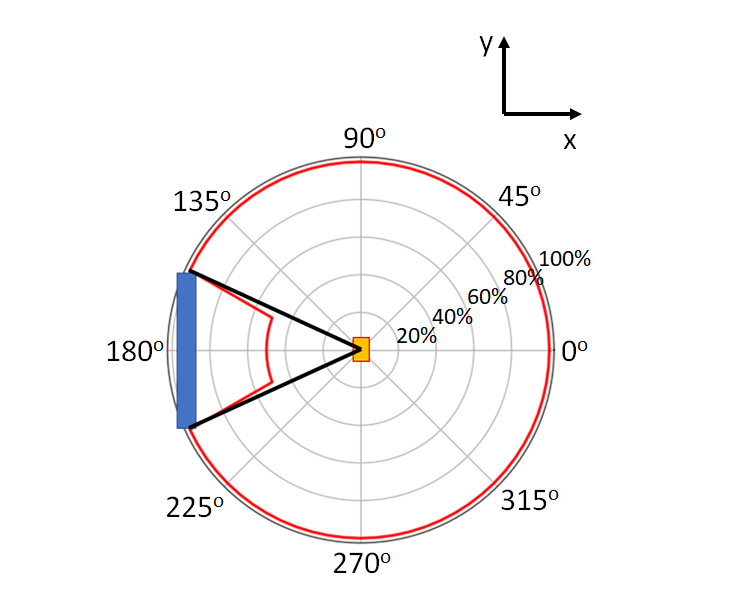
\includegraphics[width=\linewidth]{Chapter5/Figs/topDownWallPhiRedo.png}
  \captionsetup{width=.9\linewidth}
  \caption{}
  \label{subFig:TopDownCircularWallPlot}
\end{subfigure}%
\begin{subfigure}{.5\textwidth}
  \centering
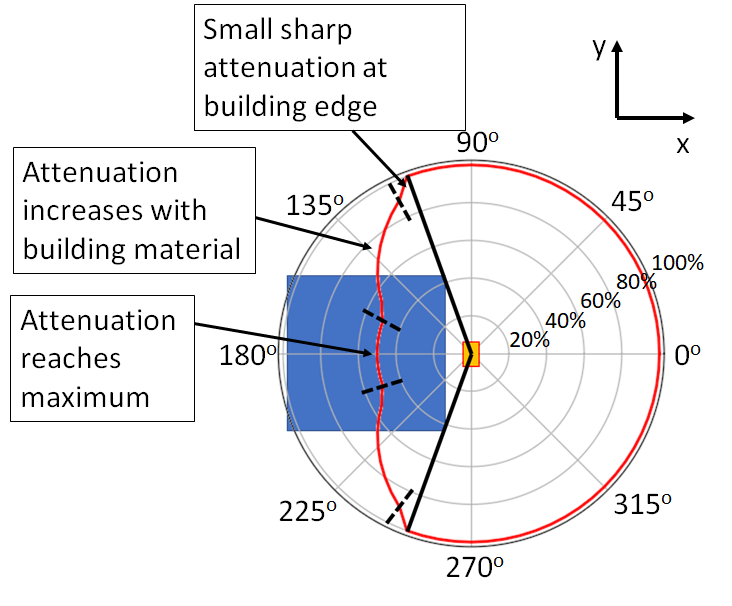
\includegraphics[width=\linewidth]{Chapter5/Figs/topDownCubePhiRedo.png}
  \captionsetup{width=.9\linewidth}
  \caption{}
  \label{subFig:TopDownCircularCubePlot}
\end{subfigure}
\caption{(a) A thin dense wall that blocks 50\,\% of cosmic $\mu$ incidence would look from a top-down perspective. A sharp drop in incidence at the edges with no further attenuation. (b) How a cube of material would block cosmic $\mu$ incidence from a top-down perspective. The amount of attenuation corresponds to the amount of material in the path of the cosmic $\mu$.}
\label{fig:TopDownCircularWallCubePlot}
\end{figure}
 
 \begin{figure}[!h]
 \centering
 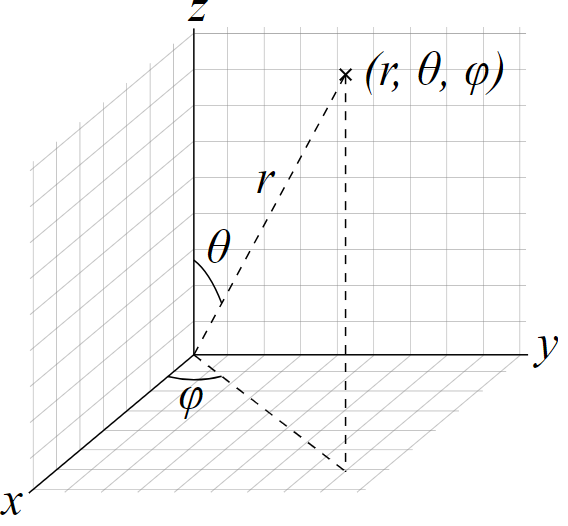
\includegraphics[width=0.3\linewidth]{Chapter5/Figs/wylfaRasterNew/sphericalPolarCoordinatesystem.png}
 \captionof{figure}{The spherical polar coordinate system is typically used in physics with the azimuthal angle denoted by $\phi$ and the polar angle denoted by $\theta$. Taken from Wikipedia \cite{wikipeidaSphericalCoordinateSystem}.} 
 \label{fig:sphericalPolarCoordinateSystem}
\end{figure}

 \begin{figure}[!h]
 \centering
 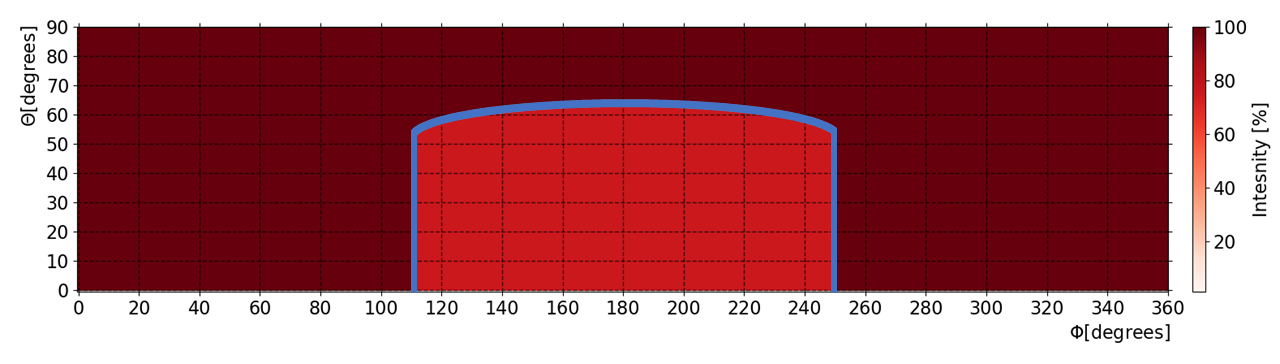
\includegraphics[width=\linewidth]{Chapter5/Figs/wylfaRasterNew/thetaVsPhiExpectedCube.png}
 \captionof{figure}{How the example seen in figure \ref{fig:TopDownCircularCubePlot} can be represented in $\theta$ and $\phi$. Assuming it's a cuboid.} 
 \label{fig:thetaVsPhiExpectedCube}
\end{figure}

For figure \ref{fig:thetaVsPhiExpectedCube} there is a slight distortion caused at the top of the building due to the projection of a hemispherical distribution onto a cuboid detector. The amount of distortion will also vary depending on the distance from the detector and the size and shape of the building in question. For example, a longer shorter building would have significantly more distortion at the top than a tall narrow building. Also, the slope of the distortion will vary depending on the position relative to the detector. Further, in figure \ref{fig:thetaVsPhiExpectedCube} the drop in intensity would not be expected to be instantaneous, there would be a gradual decrease in intensity resulting in blurred edges around the occlusion pattern or ``shadow.'' These effects will vary depending on the setup. The VIDARR prototype and upgraded VIDARR detectors for example are cuboid detectors that analyse the whole hemisphere at once, and as such can be considered as 360$^\circ$ cosmic camera rather than as a cosmic $\mu$ telescope in the strictest sense. This is an important consideration as the other cosmic $\mu$ experiments have very different experimental setups. Please see section \ref{sec:cosmicMuTelescopes} for more details.

\section{DIAPHANE $\mu$ Radiography} \label{sec:DIAPHANEmuRadiography}
The DIAPHANE detector is a plastic scintillating detector with bars with WLS fibres threaded down the centre similar to RMON and VIDARR. Instead of using silicon photomultipliers the DIAPHANE detector uses multianode PMT’s to read out the values from the WLS fibres instead  \cite{Marteau_2017}. DIAPHANE has 
% Both DIAPHANE and MU-RAY have taken tomographic data to image their surroundings. With DIAPHANE imaging La Soufriere of Guadeloupe using cosmic $\mu$ radiography as seen in figure \ref{fig:diaphaneStructualImaging} which shows the different density areas of rock relevant for volcanology \cite{Marteau_2017}.  MU-RAY has also produced similar results for mt. Vesuvius in figure \ref{fig:mtVesuviusMuRayImaging}. Though their technique and data only provide results of rock thickness in meters rather than density \cite{Ambrosino_2014}. Of more interest is figure \ref{fig:mtVesuviusMuRayTransmission} from MU-RAY which shows the ``Transmission'' method. The transmission method used in figure \ref{fig:mtVesuviusMuRayTransmission} is obtained by pointing the MU-RAY detector at the sky for a calibration period of one week then pointing the MU-RAY detector at Mt Vesuvius for one week and then taking the ratio of the two data sets \cite{Ambrosino_2014}. This approach of measuring the free sky and the blocked sky and taking the ratio of the two creates an extremely clear image because it takes the background into account. This creates a clear difference in intensity where transmission of 1 represents the free sky and transmission of 0 represents completely blocked sky. This approach is the one that will be used when analysing the Wylfa reactor site (see chapter \ref{chp:cosmicMuonTomography}) due to the effective reduction of background noise effects and the sharpness of the image it provides. 
% \\\\The DIAPHANE experimental setup seen in figure \ref{fig:DIAPHANE_deployment} shows a cosmic $\mu$ telescope with several different planes clearly analysing a very narrow field of view this helps significantly in preventing distortions via bin migration. This is also the case for the MU-RAY collaboration as seen in figure \ref{fig:muRayDetectors} the detector is also multiple flat planes. Each plane in MU-RAY is compromised of triangular prisms with WLS fibres running down the middle (see figure \ref{fig:muRaySetup}). Both MU-RAY and DIAPHANE are traditional cosmic $\mu$ telescopes as opposed to VIDARR which is an $\Bar{\nu_e}$ detector first and a cosmic $\mu$ camera second. Despite this DIAPHANE, MU-RAY, and VIDARR all use similar technology: plastic scintillating bars and WLS fibres \cite{Carroll_2018} \cite{Marteau_2017} \cite{ANASTASIO2013423}. DIAPHANE uses ``multianode PMT’s'' to read out information from the WLS fibres \cite{Marteau_2017} whereas VIDARR and MU-RAY use SiPms \cite{Carroll_2018} \cite{ANASTASIO2013423} to read out the information from the WLS fibres. 

\begin{figure}[!h]
 \centering
 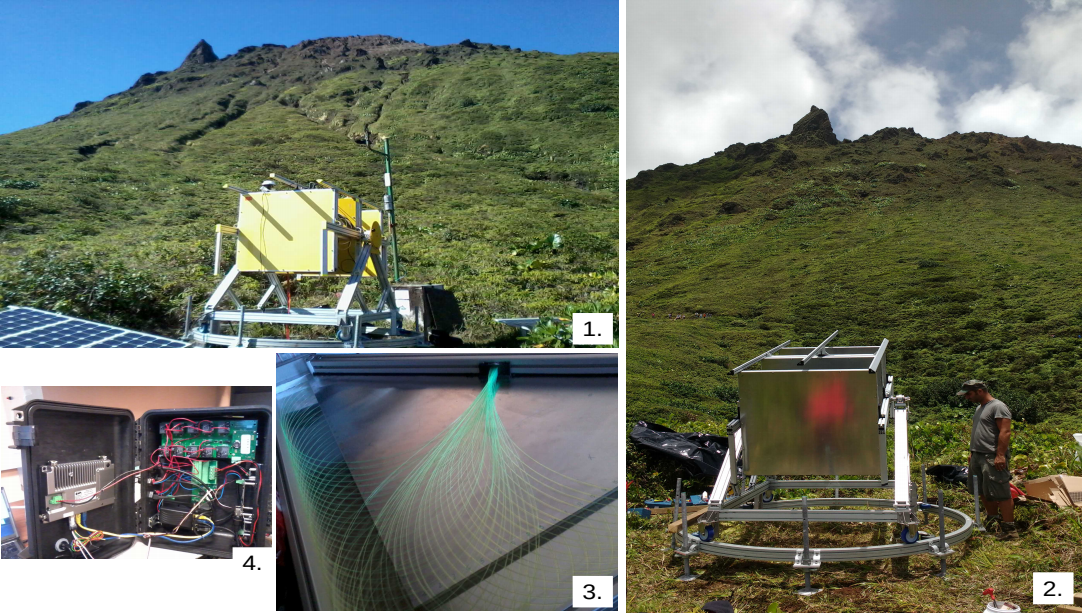
\includegraphics[width=1.0\linewidth]{Chapter5/Figs/Raster/DIAPHANE_deployment.png}
 \captionof{figure}{The deployment of the DIAPHANE detector from \cite{Marteau_2017}. DIAPHANE $\mu$ detectors upgrades. 1: the first generation 3 planes $\mu$ detector on the slope of La Soufrière of Guadeloupe (PK site). 2: the second-generation 3 planes $\mu$ detector, with a transverse segmentation divided by a factor 2, on the slope of La Soufrière of Guadeloupe (SAM site). 3: inner WLS fibres collected on a PMT cookie. 4: compact CTRL BOX with embedded hardened processing unit and electronics: common clock signal, WebRelay, Ethernet switch, Power-over-Ethernet to the wifi antenna. From \cite{Marteau_2017}.} 
 \label{fig:DIAPHANE_deployment}
\end{figure}

\begin{figure}[!h]
 \centering
 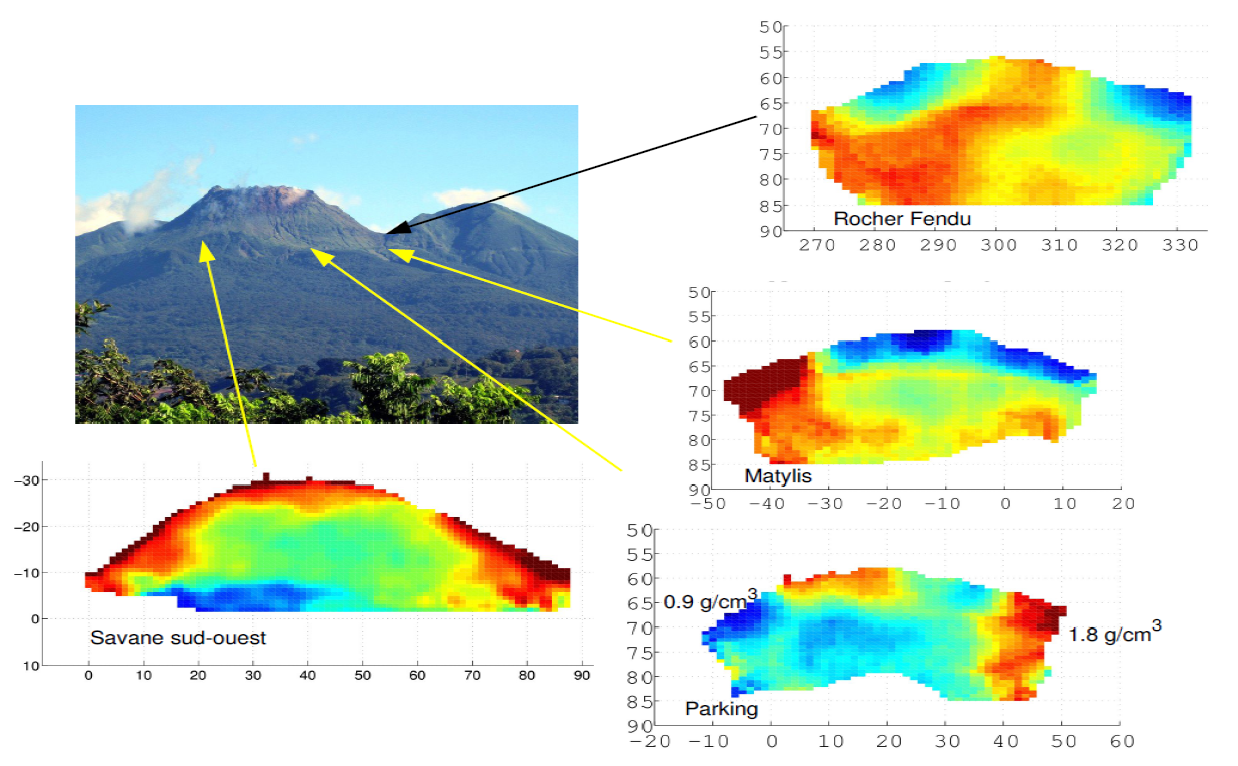
\includegraphics[width=1.0\linewidth]{Chapter5/Figs/Raster/diaphane_structuralImaging.png}
 \captionof{figure}{DIAPHANE structural imaging of the La Soufriere of Guadeloupe dome from 4 different acquisition sites around the dome. The blue areas are the less dense zones of the volcano. The red areas have the highest density. The average density extracted from all those images ranges from 1.6 to 1.8 g.cm$^{-3}$. From \cite{Marteau_2017}} 
 \label{fig:diaphaneStructualImaging}
\end{figure}

\section{MU-RAY Tomography and Transmission Method}
The MU-RAY collaboration also uses cosmic $\mu$ radiography to analyse Mt.Vesuvius. The detector uses plastic scintillator and silicon photon multipliers (SiPms) similar to that of VIDARR/RMON \cite{ANASTASIO2013423} \cite{Ambrosino_2014}. Apart from the scintillator shape which is the shape of a triangular prism in MU-RAY and the shape of a cuboid in VIDARR the two use very similar technology. The experimental setup is very similar to that of DIAPHANE with panels arranged with regular intervals (see Figure \ref{fig:muRayDetectors}). The goals of DIAPHANE and MU-RAY are the same -- to image the interior of volcanoes. MU-RAY even has low power requirements so solar power can be used in remote locations \cite{ANASTASIO2013423}. 

\begin{figure}[!h]
 \centering
 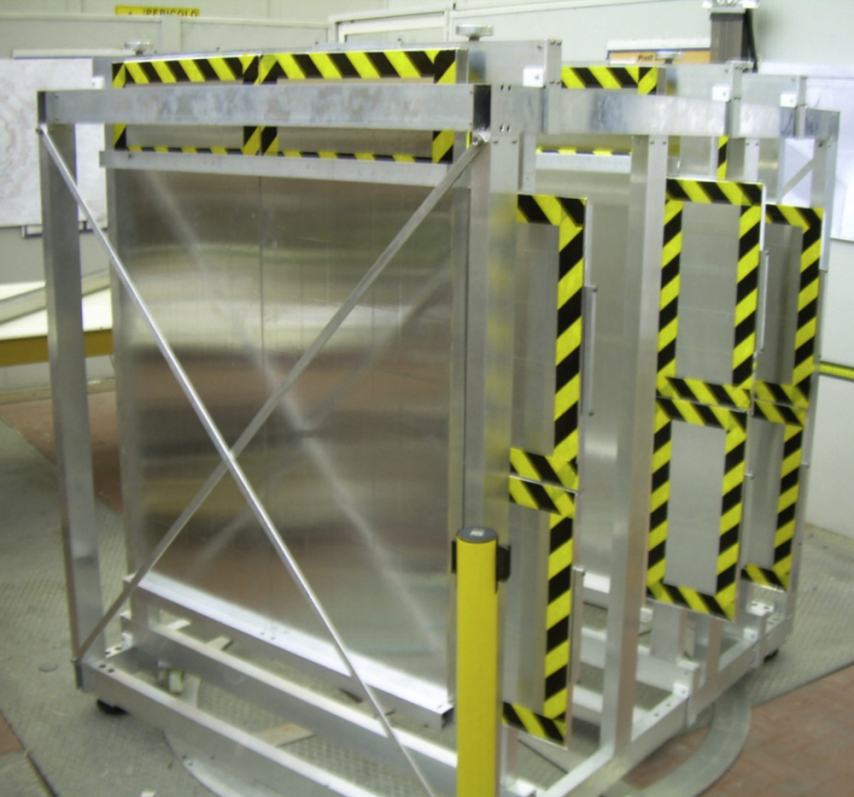
\includegraphics[width=0.5\linewidth]{Chapter5/Figs/Raster/muRayDetectors.png}
 \captionof{figure}{The MU-RAY detector frame with the three X–Y planes mounted. The frame can be oriented using the rotating platform visible at the bottom. From \cite{ANASTASIO2013423}} 
 \label{fig:muRayDetectors}
\end{figure}

The limits of $\mu$ radiography is clearly demonstrated by figure \ref{fig:mtVesuviusMuRayImaging}. Whilst the MU-RAY detector was deployed with no obstructions and had a deployment time of $\sim$ 1 month and was elevated by 800\,m reducing atmospheric scattering the outline of Mt.Vesuvius is still faint. Whilst the increase in rock thickness is clearly visible in figure \ref{fig:mtVesuviusMuRayImaging} there are no clear defining features. These results are in stark contrast to the DIAPHANE results at Guadeloupe (figure \ref{fig:diaphaneStructualImaging}) which show clear interior structural imaging of a volcano. Whilst the technology of DIAPHANE and MU-RAY is not identical they are very similar. DIAPHANE has better energy reconstruction due to the multianode PMT’s as opposed to the SiPms used in MU-RAY \cite{Marteau_2017}, \cite{ANASTASIO2013423}. However, the spatial reconstruction should be superior in MU-RAY as the segments in DIAPHANE have a cross section of 5\,cm $\times$ 1\,cm (5\,cm$^2$) \cite{MARTEAU201223}, whereas the MU-RAY triangular cross section has a base width of 3.3\,cm and height 1.7\,cm (2.805\,cm$^2$). As a result the blurry resolution in figure \ref{fig:mtVesuviusMuRayImaging} is surprising and leads to the conclusion that the 5 year deployment time for DIAPHANE is the main reason for the sharper resolution in figure \ref{fig:diaphaneStructualImaging}.

\begin{figure}[!h]
 \centering
 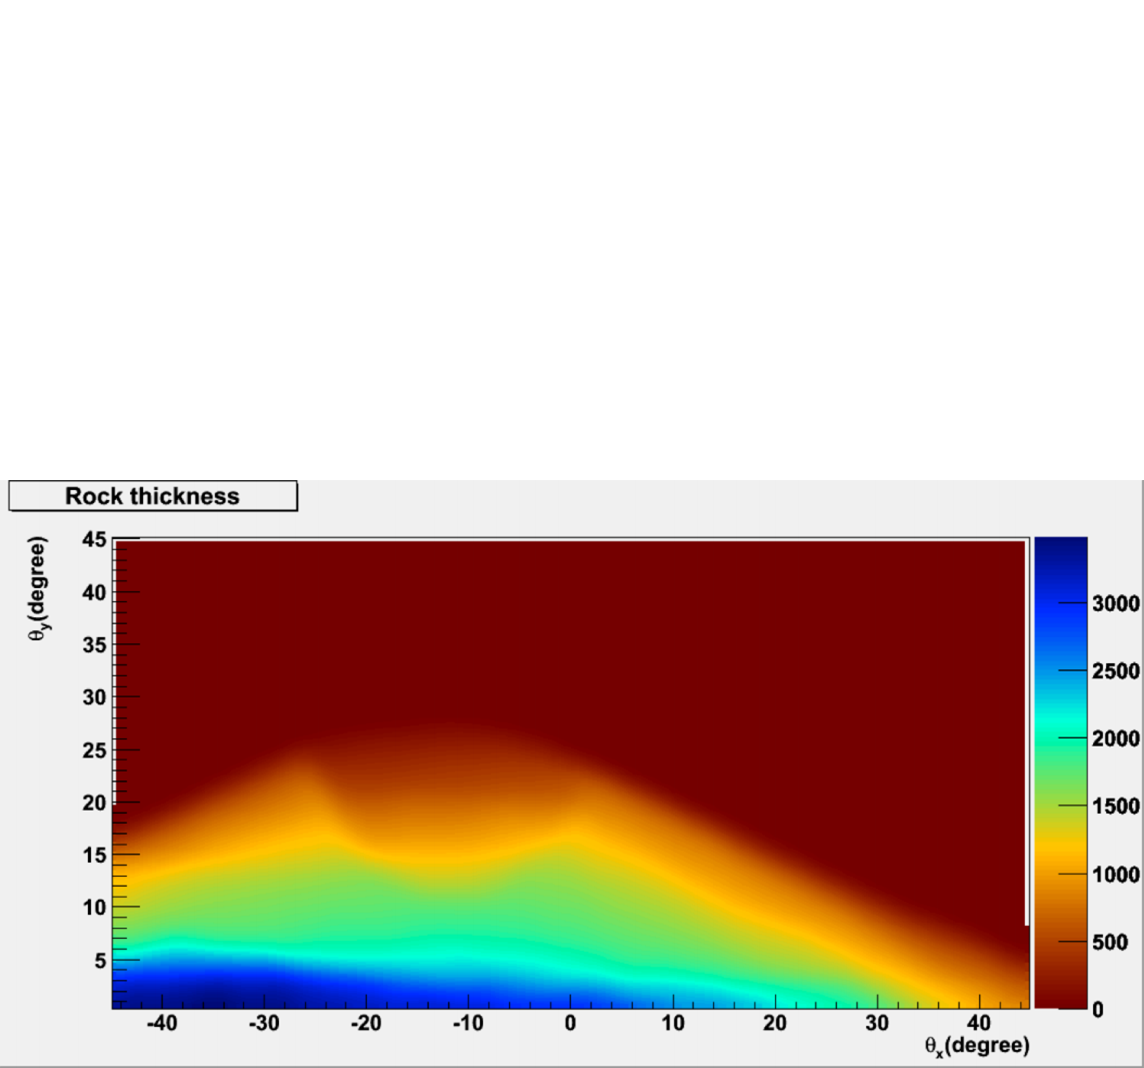
\includegraphics[width=0.7\linewidth]{Chapter5/Figs/Raster/mtVesuviusMuRayImaging.png}
 \captionof{figure}{MU-RAY telescope analysing Vesuvius rock thickness, expressed in m, as seen from the observation point at $\sim$ 800 m altitude. With data taken over a month period of $\sim$ 1 month. From \cite{Ambrosino_2014}.} 
 \label{fig:mtVesuviusMuRayImaging}
\end{figure}

As a result of their limited deployment time the MU-RAY collaboration took $\sim$ 1 week to image Mt.Vesuvius using a different technique. The transmission technique. The results are shown in figure \ref{fig:mtVesuviusMuRayTransmission} whilst this data set has $\sim$ 4 times live time data than for figure \ref{fig:mtVesuviusMuRayImaging} the results are much clearer. The transmission method takes the ratio of the unblocked vertical sky with the area where Mt.Vesuvius is located \cite{Ambrosino_2014}. The effect is so significant because the acceptance and efficiency dependencies are cancelled out as such when normalised to the acquisition run the free sky zone common to both histograms should be close to 1 \cite{Ambrosino_2014}. This is especially useful for cosmic $\mu$ tomography for RMON and VIDARR as the field of view is much wider 

\begin{figure}[!h]
 \centering
 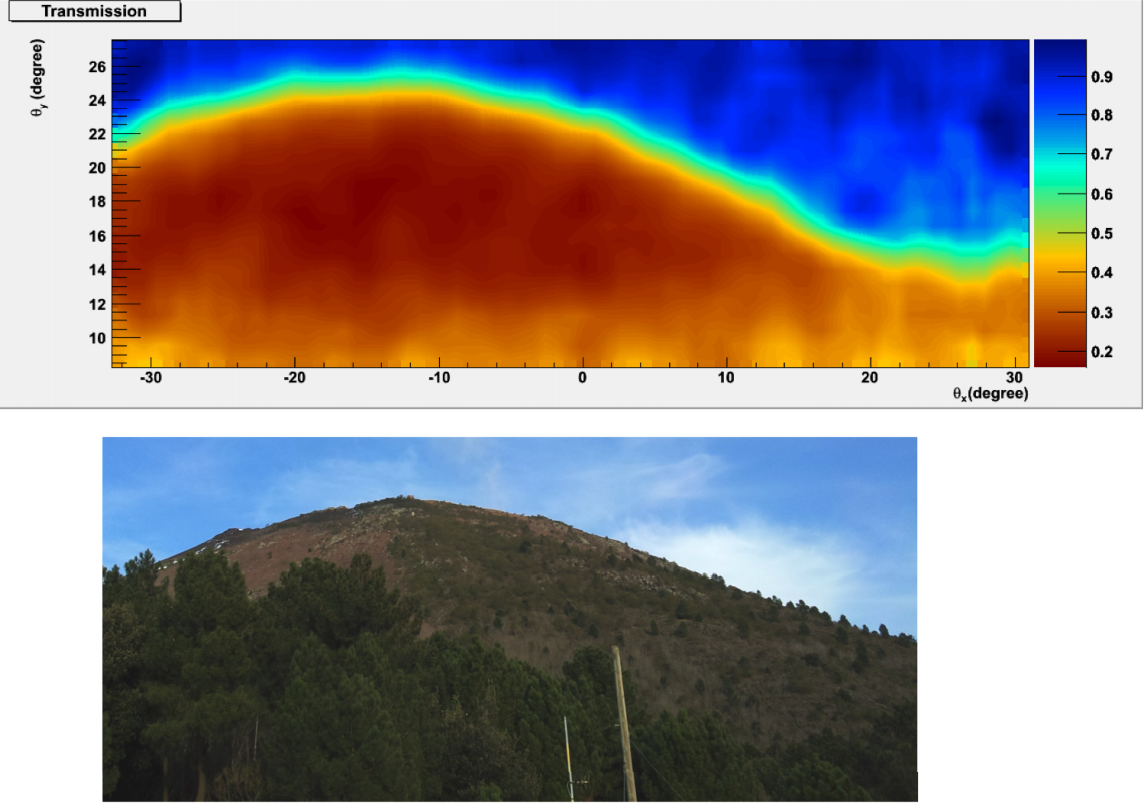
\includegraphics[width=0.7\linewidth]{Chapter5/Figs/Raster/mtVesuviusMuRayTransmission.png}
 \captionof{figure}{MU-RAY data from Vesuvius. Top: the transmission histogram of Mt Vesuvius after one week of data taking. Bottom: a picture of Mt Vesuvius taken by the telescope observation point. Taken over a period of $\sim$ 1 week. From  \cite{Ambrosino_2014}.} 
 \label{fig:mtVesuviusMuRayTransmission}
\end{figure}
